% % % % % % % % % % % % % % % % % % % % % % % % % % % % % % % % % % % % % % % % % % % %
%                                                                                     %
% Short Sectioned Assignment LaTeX Template Version 1.0 (5/5/12)                      %
% This template has been downloaded from: http://www.LaTeXTemplates.com               %
%                                                                                     %
% Original author:  Frits Wenneker (http://www.howtotex.com)                          %
%                                                                                     %
% Modified by: Fco Javier Sueza Rodríguez (fcosueza@disroot.org)                      %
%                                                                                     %
% Changes:                                                                            %
%	    - Custom Chapters, Sections and Subsections (titlesec package)                %
%           - Document type scrbook (oneside)                                         %
%           - Use babel-lang-spanish package and marvosym                             %
%           - Use hyperref, enumitem, tcolorbox and glossaries packages               %
%           - Use Time New Roman (mathptmx), Helvetic and Courier fonts               %
%                                                                                     %
% License: CC BY-NC-SA 3.0 (http://creativecommons.org/licenses/by-nc-sa/3.0/)        %
%                                                                                     %
% % % % % % % % % % % % % % % % % % % % % % % % % % % % % % % % % % % % % % % % % % % %

%-----------------------------------------------%
%	              Packages                  %
%-----------------------------------------------%

\documentclass[paper=a4, fontsize=11pt, oneside]{scrbook}

% ---- Text Input/Output ----- %

\usepackage[T1]{fontenc}
\usepackage[utf8]{inputenc}
\usepackage{mathptmx}
\usepackage[scaled=.92]{helvet}
\usepackage{courier}
\usepackage[indent=12pt]{parskip}

\usepackage{geometry}
\geometry{verbose,tmargin=3cm,bmargin=3cm,lmargin=2.6cm,rmargin=2.6cm}

% ---- Language ----- %

\usepackage[spanish]{babel}
\usepackage{marvosym}

% ---- Another packages ---- %

\usepackage{amsmath,amsfonts,amsthm}
\usepackage{graphics,graphicx}
\usepackage{titlesec}
\usepackage{fancyhdr}
\usepackage{tcolorbox}
\usepackage{hyperref}
\usepackage{enumitem}
\usepackage[automake]{glossaries}

%--------------------------------------------------------------------%
%                      Customizing Document                          %
%--------------------------------------------------------------------%


% ----------- Custom Chapters, Sections and Subsections -------------- %

\titleformat{\chapter}[display]
			{\bfseries\Huge}
			{Tema \ \thechapter} {0.5ex}
			{\vspace{1ex}\centering}

\titleformat{\section}[hang]
			{\bfseries\Large}
			{\thesection}{0.5em}{}

\titleformat{\subsection}[hang]
			{\bfseries\large}
			{\thesubsection}{0.5em}{}

\titleformat{\subsubsection}[hang]
			{\bfseries\large}
			{\thesubsubsection}{0.5em}{}

\hypersetup{
    colorlinks=true,
    linkcolor=black,
    urlcolor=magenta
}

% ------------------- Custom heaaders and footers ------------------- %

\pagestyle{fancyplain}

\fancyhead[]{}
\fancyfoot[L]{}
\fancyfoot[C]{}
\fancyfoot[R]{\thepage}

\renewcommand{\headrulewidth}{0pt} % Remove header underlines
\renewcommand{\footrulewidth}{0pt} % Remove footer underlines

\setlength{\headheight}{13.6pt} % Customize the height of the header

% --------- Numbering equations, figures and tables ----------------- %

\numberwithin{equation}{section} % Number equations within sections
\numberwithin{figure}{section} % Number figures within sections
\numberwithin{table}{section} % Number tables within sections

% ------------------------ New Commands ----------------------------- %

\newcommand{\horrule}[1]{\rule{\linewidth}{#1}} % Create horizontal rule command


%----------------------------------------------------------------------------------------
%	TÍTULO Y DATOS DEL ALUMNO
%----------------------------------------------------------------------------------------

\title{
\normalfont \normalsize
\textsc{{\bfseries Curso 2023-2024} \\ Ciclo Superior de Desarrollo de Aplicaciones Web \\ IES Aguadulce} \\ [25pt]
\horrule{0.5pt} \\[0.4cm]
\huge Programación \\
\horrule{0.5pt} \\[0.4cm]
}

\author{Francisco Javier Sueza Rodríguez}
\date{\normalsize\today}

%----------------------------------------------------------------------------------------
%                                     DOCUMENTO
%----------------------------------------------------------------------------------------
\makeglossaries
\loadglsentries{glossary.tex}

\begin{document}

\maketitle

\newpage

\tableofcontents

\listoffigures

%\listoftables

\newpage

\chapter{Introducción a la Programación}

En esta primera unidad vamos a estudiar los conceptos básicos de la programación de aplicaciones. Comenzaremos estudiando que es la programación, que técnicas podemos emplear, que herramientas podemos utilizar y cual es objetivo que pretendemos alcanzar. Analizaremos las diferentes paradigmas de programación  existentes, identificaremos las fases del desarrollo de un programa.

Una vez realizada una introducción general, detallaremos las características relevantes de los principales lenguajes de programación, para a continuación centrarnos en el lenguaje que vamos a usar durante toda esta asignatura, \textbf{Java}, dando a conocer también que herramientas podemos usar para que nuestro desarrollo sea más sencillo con este lenguaje.

\section{Programas: Buscando una Solución}
La principal razón que mueve  a una persona hacia el aprendizaje de la programación es utilizar el ordenador como una herramienta para resolver diferentes problemas. Al igual que en la vida real, las búsqueda y obtención de una solución requiere de una serie de \textbf{pasos fundamentales}.

\begin{figure}[H]
    \centering
    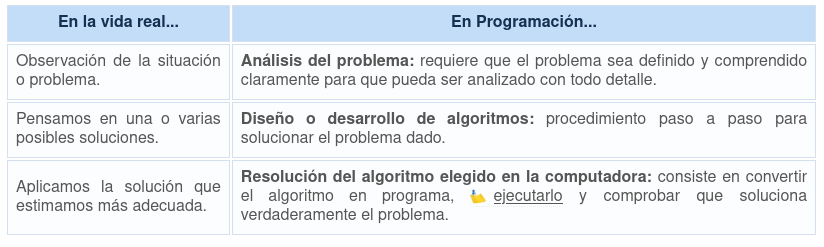
\includegraphics[scale=0.70]{pasos-problemas.png}
    \caption{Pasos para la resolución de un problema}
\end{figure}

Para que una \textbf{solución} se considere \textbf{correcta} tiene que tener principalmente dos características:

\begin{itemize}
    \item \textbf{Corrección y Eficacia}: si resuelve el problema de forma adecuada.
    \item \textbf{Eficiencia}: si lo realiza en un tiempo mínimo y con un uso óptimo de los recursos del sistema.
\end{itemize}

Para construir esta solución, hay que tener en cuenta algunos conceptos ligados a la programación, como son:

\begin{enumerate}
    \item \textbf{Abstracción}: se trata de realizar una análisis del problema para descomponerlo en problemas más pequeños y de menos complejidad de manera precisa. \textbf{Divide y Vencerás}: es una filosofía general para resolver problemas y de aquí que no solo forme parte del vocabulario informático, sino que también se utiliza en otros muchos ámbitos.

    \item \textbf{Encapsulación}: consiste en ocultar la información de un objeto o función de forma que se pueda implementar de diferentes maneras sin que esto afecte al resto de objetos.

    \item \textbf{Modularidad}: estructuraremos cada parte en módulos independientes, cada uno con su función correspondiente.
\end{enumerate}

Todo estos conceptos, deberemos tenerlos en cuenta a la hora de analizar el problema, para llegar a un solución lo más óptima posible.

\subsection{Algoritmos y Programas}
Una vez realizado el análisis del problema, tenemos que diseñar y desarrollar un \textbf{algoritmo} adecuado que pueda solucionarlo. Pero, ¿que es un algoritmo?

Un \textbf{algoritmo} es una secuencia ordenada de pasos, descrita sin ambigüedades, que conducen a la solución de un problema.

Los algoritmos deben ser \textbf{independientes} de los \textbf{lenguajes de programación} y de las \textbf{computadoras} donde se ejecutan, de forma que puedan implementarse sobre cualquier ordenador empleando cualquier lenguaje de programación. Esto facilita que una misma solución pueda emplearse para el mismo problema en diferentes dispositivos.

La \textbf{diferencia} entre un algoritmo y un \textbf{programa} es que en este último lo pasos deben escribirse en un \textbf{lenguaje de programación concreto} para que pueda ser ejecutado en el ordenador y así obtener la solución deseada.

Los \textbf{lenguajes de programación} son solo un medio para expresar el algoritmo y el ordenador un procesador para ejecutarlo. El diseño de algoritmos es una tare que requiere de la creatividad y conocimientos de las técnicas de programación del programador, así, diferentes programadores pueden desarrollar diferentes algoritmos para resolver un mismo problema.

Las principales \textbf{características} que debe cumplir un \textbf{algoritmo} son:

\begin{itemize}
    \item Debe ser \textbf{preciso} e indicar el orden en el que se realiza cada paso.
    \item Debe estar \textbf{bien definido}, si se ejecuta dos o más veces, debemos obtener el mismo resultado.
    \item Debe ser \textbf{finito}, teniendo un número de pasos bien determinado.
\end{itemize}

Cuando los problemas complejos, debemos descomponer estos en subproblemas más simples, y estos a su vez en otros más pequeños. Es lo que se conoce como \textbf{diseño descendente} o \textbf{diseño modular} y se basa en el lema \textbf{Divide y Vencerás}.

Para \textbf{representar gráficamente} los algoritmos tenemos diferentes herramientas que nos ayudarán a describir su comportamiento de una forma precisa y genérica, que nos facilitará la implementación del algoritmo en diferentes lenguajes de programación. Las principales herramientas que tenemos son:

\begin{itemize}
    \item \textbf{Diagramas de Flujo}: esta técnica utiliza símbolos gráficos para representar el flujo de ejecución del algoritmo y suelen ser empleados en la fase de análisis.
    \item \textbf{Pseudocódigo}: se basa en el uso de palabras clave en lenguaje natural, representando las constantes, variables y otras estructuras de programación de forma escrita. Es la técnica mas utilizada actualmente.
    \item \textbf{Tablas de Decisión}: es un tabla que representa las diferentes condiciones del problema con sus respectivas acciones. Suele ser una técnica de apoyo a pseudocódigo cuando existen circunstancias condicionales complejas.
\end{itemize}

\section{Fases de la Programación}
Sea cual sea el estilo que escojamos para resolver el problema, deberemos realizar el proceso aplicando un método a nuestro trabajo. Así, el \textbf{proceso de creación de software} se puede dividir en las siguientes \textbf{fases}:

\begin{itemize}
    \item \textbf{Fase de resolución del problema}
    \item \textbf{Fase de implementación}
    \item \textbf{Fase de explotación y mantenimiento}
\end{itemize}

En los siguientes puntos, analizaremos cada una de estas fases.

\subsection{Resolución del Problema}
Esta es la primera fase del desarrollo del programa, para la cuál deberá estar bien definido cual es el problema que se quiere solucionar y tener un comprensión clara de éste para poder realizar su análisis y diseño. Esta fase se puede dividir en \textbf{dos etapas}:

\begin{enumerate}
    \item \textbf{Etapa de Análisis}:

    En esta primera etapa se debe analizar el problema, lo que nos va a indicar las especificaciones y requisitos que la aplicación debe cumplir. Para llevar esto acabo, se deberán realizar diferentes entrevistas entre el programador y el cliente/usuario para precisar cuales son las características que debe tener la aplicación, especificando, entre otras cosas, los procesos y estructuras que deberá tener ésta. La creación de \textbf{prototipos} será muy útil en esta fase para saber con mayor exactitud los puntos a tratar.

    Esta etapa proporcionará una idea general de lo que se solicita, realizando sucesivos refinamientos posteriormente que servirá para determinar cual es la información que ofrecerá la resolución del problema y que datos son necesarios para resolver este.

    \item \textbf{Etapa de Diseño}:

    En esta tapa se convierte la especificación de la etapa de análisis en un diseño más detallado que define el comportamiento o la secuencia lógica de instrucciones capaz de resolver el problema planteado. Estos pasos sucesivos, constituyen lo que ya hemos definido como algoritmo.

    Antes de pasar a la implementación del algoritmo, tenemos que tener claro que la solución que se propone es la adecuada. Para ello, toda solución necesitará de la \textbf{prueba} o \textbf{traza} del programa. Este procedimiento consistirá en el seguimiento paso a paso de cada instrucción del algoritmo utilizando los datos correctos. Si la solución aportada contiene errores, deberemos volver a la etapa de análisis, si no, podremos pasar a la fase de implementación.
\end{enumerate}

\subsection{Implementación}


% Bibliography

\newpage
\addcontentsline{toc}{chapter}{Bibliografía}
\bibliography{citas}
\bibliographystyle{unsrt}

\end{document}